\section{Data Preparation} 
Our data come from the judgement documents published on China Judgements Online. The Chinese government has been publishing the judgement documents on it since 2013\footnote{There are also judgements before 2013.}. We randomly choose 50,000 judgements as training data, 5,000 for validation and 5,000 for test. To ensure enough training data for each charge, we keep the charges that appear more than 50 times in our training data. As for law articles, we only keep articles in Chinese Criminal Law. In our final dataset, there are 50 distinct charges and 321 distinct articles. About 3.6\% cases contain more than one charges, and 94.2\% cases contain more than one law articles. The fact description part of each judgement document contains 383 words, and 14 sentences on average.

\begin{figure*}[htbp]
\begin{center}
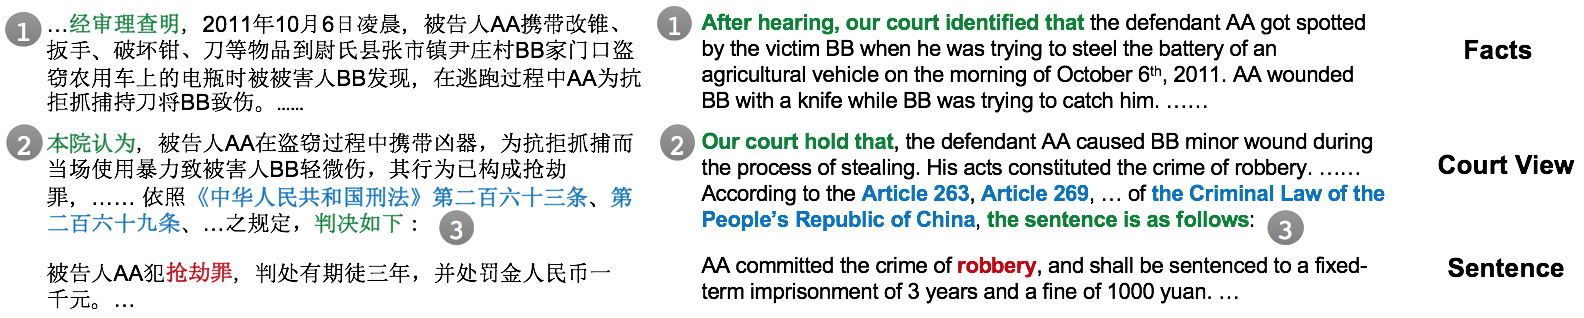
\includegraphics[width=0.97\textwidth]{figures/case.png}	
\caption{Example Judgement Document of a Chinese Criminal Case}
\label{fig_example_case}
\end{center}
\end{figure*}

One of the judgements is shown in Figure \ref{fig_example_case}. Although there does not exist a strict rule for formatting a judgement document, we can still discover some patterns in it. A typical judgement document often starts with a brief description of the procedure followed before the judgement, from the start of the prosecution until the case is decided. The procedure is often followed by the facts of the case. After that, the court will conclude the case and provide relevant law articles that can be applied to the case. Finally, the sentence part will list the charges of the defendant along with corresponding penalties. 

We find that the fact description part often starts with the clause 经审理查明$\ $(after hearing, our court identified that), and the court view part often starts with the clause 本院认为$\ $(our court hold that). Therefore we extract the texts between these two clauses as fact description. Since the mentions of charges do not have many variations in judgement documents, we manually build a list that contains the possible variations of each charge based on a public criminal charge list\footnote{\url{http://china.findlaw.cn/zuiming/}}. Then the list is used to find accusation mentions in the sentence part with exact matching. As for law articles, since the article is often mentioned in a fixed patterns, we simply use regular expressions to identify the article mentions. 

Note that we only keep the cases with only one defendant. We discard cases with multiple defendants because it is hard to separately relate each defendant to his (or her) corresponding facts, articles and charges due to the unstructured nature of the judgement document.